%% margin: The margin between outer edge of the poster and the edge of the paper; i.e. ultimate margin
%% innermargin: The margin from the edge of the poster edge to the outermost edge of the blocks; i.e. content margin
%% colspace (horitzontal collumn space?) needs to be high before it's noticable
% innermargin was 40pt, idk what's printable
\documentclass[25pt, a0paper, portrait, margin=0pt, innermargin=40pt, colspace=40pt, blockverticalspace=45pt]{tikzposter}

% disable hypnetation
%% \usepackage[none]{hyphenat} % behaves kinda odd, requires multiple compiles?
\usepackage{babel}

\usepackage{blindtext}
\usepackage{xcolor}
\usepackage{multicol}
\usepackage{fix-cm}
\usepackage{stackengine}
\usepackage[utf8]{inputenc}
\usepackage{enumitem}

% figures
\usepackage{graphicx}
\usepackage{float}
\usepackage{caption}
\DeclareCaptionFormat{postersize}{\fontsize{30}{36}\selectfont#1#2#3}
\captionsetup{format=postersize}
\usepackage{tabularx}
%% \usepackage{wrapfig} % doesn't work so far

% tikz
\usepackage{standalone}
\usetikzlibrary{positioning}
\usetikzlibrary{shapes.geometric}
\usetikzlibrary{calc}
\usetikzlibrary{decorations.pathreplacing}
%% \usetikzlibrary{arrows}
\usetikzlibrary{arrows.meta}
\newcommand\vcdots{\;\stackMath\stackinset{c}{0pt}{c}{0.6ex}{\vdots}{\vphantom{-}}\;}

% Table packages
\usepackage{booktabs}

% Math
\usepackage{amssymb}
\usepackage{amsmath}
%% sans serif math font
\usepackage[cmbright]{sfmath}
%% \usepackage[EULERGREEK]{sansmath}
%% \sansmath


% Bibliography
%% \usepackage[ backend=biber, sorting=none, maxcitenames=2, natbib]{biblatex}
%% \addbibresource{poster.bib}
\usepackage[square,numbers, sort&compress]{natbib}
\bibliographystyle{short}
%% \bibliographystyle{unsrtnat}
%% \bibliographystyle{agsm}
% this only redefines the citations in text
\renewcommand{\bibnumfmt}[1]{\textbf{[#1]} \,}
% remove "References" heading in natbib
\renewcommand{\bibsection}{}


\usepackage[]{fontspec}
\defaultfontfeatures{Mapping=tex-text,Scale=MatchLowercase}
\setmainfont{Open Sans}
%% \usepackage[T1]{fontenc}
%% this scaling feature is pretty handy
%% \usepackage[default,scale=0.79]{opensans}

%% \usepackage[default]{lato}
%% \usepackage[T1]{fontenc}

%% \renewenvironment{tikzfigure}[1][]{
%%   \begin{center}
%%   \hspace{0pt}
%%   \vfill
%%   }{
%%   \vfill
%%   \hspace{0pt}
%%   \end{center}
%% }

%% \meaning\tikzfigure

% based on "Minimal" blockstyle
% body ofsett 1 is nice bc of the titleless innerblock "glitch"
% (see stackexchange link below)
\defineblockstyle{eccv2}{
    titlewidthscale=1, bodywidthscale=1, titlecenter,
    titleoffsetx=0pt, titleoffsety=0pt, bodyoffsetx=0pt, bodyoffsety=0pt,
    bodyverticalshift=-6pt, roundedcorners=6, linewidth=0.42cm, % same as innersep
    titleinnersep=1cm, bodyinnersep=0.21cm
}{
    \begin{scope}[line width=\blocklinewidth, rounded corners=\blockroundedcorners]
      %% uncomment the ifs for different titleless look
       \ifBlockHasTitle %
           % box outline
           \draw[draw=eccvgrayblue, fill=white]
               (blockbody.south west) rectangle (blocktitle.north east);
           % title rectangle
           \fill[eccvgrayblue]
               (blocktitle.south west) rectangle (blocktitle.north east);
        \fi
    \end{scope}
}

% Consider making the line either blue or gray
\defineblockstyle{eccv2optimizations}{
    titlewidthscale=1, bodywidthscale=1, titlecenter,
    titleoffsetx=0pt, titleoffsety=0pt, bodyoffsetx=0pt, bodyoffsety=0pt,
    bodyverticalshift=-6pt, roundedcorners=6, linewidth=0.42cm, % same as innersep
    titleinnersep=1cm, bodyinnersep=0.21cm
}{
    \begin{scope}[line width=\blocklinewidth, rounded corners=\blockroundedcorners]
      % box outline
      \draw[draw=eccvgrayblue, fill=none]
      	(blockbody.south west) rectangle (blocktitle.north east);
      % title rectangle
      \fill[eccvgrayblue]
      	(blocktitle.south west) rectangle (blocktitle.north east);
      % seperator line
      \path (blockbody.south) 
      % sorta add these corrdinates/values to the start
      +(0.0cm,6cm) coordinate (c1);
      \path (blockbody.north)
      +(0.0cm, -1cm) coordinate (c2);
      %% \draw [line width=0.42cm,eccvgrayblue, dashed, dash pattern=on 20pt off 20pt] (blockbody.south) -- (blockbody.north);
      \draw [line width=0.15cm,eccvgrayblue] (c1) -- (c2);
    \end{scope}
}

\defineblockstyle{reference}{
    titlewidthscale=1, bodywidthscale=1, titlecenter,
    titleoffsetx=0pt, titleoffsety=0pt, bodyoffsetx=0pt, bodyoffsety=0pt,
    bodyverticalshift=0pt, roundedcorners=0, linewidth=0.0cm, % same as innersep
    titleinnersep=0cm, bodyinnersep=0pt % matches innerbody style
}{}

% the titleoffsety is important, see
% https://tex.stackexchange.com/questions/447378/tikzposter-leaves-a-gap-in-empty-innerblock-title
\defineinnerblockstyle{eccvinner}{
    titlewidthscale=1, bodywidthscale=1, titlecenter,
    titleoffsetx=0pt, titleoffsety=-0pt, bodyoffsetx=0pt, bodyoffsety=0pt,
    bodyverticalshift=0pt, roundedcorners=0, linewidth=0.0cm,
    titleinnersep=0pt, bodyinnersep=25pt
}{
    \begin{scope}[line width=\innerblocklinewidth, rounded corners=\innerblockroundedcorners]
       \ifInnerblockHasTitle %
           \filldraw[innerblockbodybgcolor]
               (innerblockbody.south west) rectangle (innerblocktitle.north east);
       \else
             \filldraw[innerblockbodybgcolor]
                 (innerblockbody.south west) rectangle (innerblockbody.north east);
        \fi
    \end{scope}
}

\defineinnerblockstyle{eccvinneroptimizations}{
    titlewidthscale=1, bodywidthscale=1, titlecenter,
    titleoffsetx=0pt, titleoffsety=-0pt, bodyoffsetx=0pt, bodyoffsety=0pt,
    bodyverticalshift=0pt, roundedcorners=0, linewidth=0.0cm,
    titleinnersep=0pt, bodyinnersep=25pt
}{}

% Redefine block title stuff
\usepackage{xpatch}
\xpatchcmd{\block}{\bf\LARGE\color{blocktitlefgcolor}}{\bfseries\huge\color{eccvblue}}{}{}
\xpatchcmd{\innerblock}{\bf \color{innerblocktitlefgcolor}}{\bfseries\color{eccvblue}}{}{}
% remove space that empty innerblock title leaves behind
\makeatletter
\xpatchcmd{\innerblock}{\node[minimum width=\TP@innerblocktitlewidth, minimum height=\TP@innerblocktitleheight, anchor=center] (innerblocktitle)}{\node[inner sep=0pt, minimum width=\TP@innerblocktitlewidth, minimum height=\TP@innerblocktitleheight, anchor=center] (innerblocktitle)}{}{}
\makeatother

%% redo font stuff here I guess
%% Inner body text style
\xpatchcmd{\block}{#3}{\fontsize{30}{36}#3}{}{}

\definecolor{eccvlightblue}{HTML}{009EE0}
\definecolor{eccvlightblued}{HTML}{6898be}
% more gray blue ish but makes a good background color
% combine with background titles in like light blue?
\definecolor{eccvgrayblue}{HTML}{E2F1F9}
\definecolor{eccvsuperlightblue}{HTML}{F5F9FF}
%% \definecolor{eccvgrayblue}{HTML}{D7FFFF}
\definecolor{eccvblue}{HTML}{045494}
\definecolor{eccvdarkblue}{HTML}{023258}
%% \definecolor{lightgrey}{HTML}{777777}
\definecolor{lightgrey}{HTML}{CCCCCC}

%% define a gray for all the blocks (iterm gray?) and github blue
%% Primary colors are iTerm gray (to be combined with blue backgrounds?)
%% black and eccv blue
\definecolorstyle{eccvblue} {
\definecolor{colorOne}{named}{white}
\definecolor{colorTwo}{named}{eccvlightblue}
\definecolor{colorThree}{named}{eccvblue}
}{
% Background Colors
\colorlet{backgroundcolor}{white}
\colorlet{framecolor}{black}
% Title Colors
\colorlet{titlefgcolor}{colorThree}
\colorlet{titlebgcolor}{colorOne}
% Block Colors
\colorlet{blocktitlebgcolor}{colorThree}
\colorlet{blocktitlefgcolor}{white}
\colorlet{blockbodybgcolor}{white}
\colorlet{blockbodyfgcolor}{black}
% Innerblock Colors
\colorlet{innerblocktitlebgcolor}{white}
\colorlet{innerblocktitlefgcolor}{black}
\colorlet{innerblockbodybgcolor}{colorThree!30!white}
\colorlet{innerblockbodyfgcolor}{black}
% Note colors
\colorlet{notefgcolor}{black}
\colorlet{notebgcolor}{colorTwo!50!white}
\colorlet{noteframecolor}{colorTwo}
}



\definetitlestyle{simpletitle}{
width=807mm, roundedcorners=0, linewidth=0pt, innersep=0pt,
titletotopverticalspace=40pt, titletoblockverticalspace=45pt}{% more precise?
\begin{scope}[line width=\titlelinewidth, rounded corners=\titleroundedcorners]
\draw[color=white, fill=titlebgcolor] % notice the white hack
(\titleposleft,\titleposbottom) rectangle (\titleposright,\titlepostop);
\end{scope}
}

\newcommand\boldblue[1]{\textcolor{eccvblue}{\textbf{#1}}}
\newcommand\markblue[1]{\textcolor{eccvblue}{{#1}}}


\tikzposterlatexaffectionproofoff

% Make the title layout horizontal instead of vertical, as in Tom's Example?
% that way you can squeeze more information in
\title{SUBITIZING WITH VARIATIONAL AUTOENCODERS}
\author{Rijnder Wever, Tom Runia}
\date{\today}
\institute{University of Amsterdam}
\titlegraphic{
\includegraphics[width=3.6cm]{UVA-plain}}

\usecolorstyle[colorOne=white,colorTwo=black,colorThree=eccvblue]{eccvblue}
\usetitlestyle{simpletitle}

\settitle{
    %% \begin{multicols}{2}
    %% \setstackgap{L}{1em}
    %% \vspace*{-1\topskip plus 1fill}
  	\noindent\begin{minipage}{0.71\linewidth}
    \vbox{
      \color{titlefgcolor} {\bfseries \fontsize{80}{96} \selectfont \@title \par}
      \vspace*{1.0em}
      % The two different colors in the title are really not that nice
      \color{titlefgcolor} {\huge \@author}}
    %% \vspace*{\fill}
    %% \columnbreak
    \end{minipage}
    \hfill%
    \begin{minipage}{0.29\linewidth}
      \vspace*{-10pt}
      \noindent\begin{minipage}{0.6\textwidth}\raggedleft
        \@titlegraphic
      \end{minipage}
      \hfill%
      \begin{minipage}{0.4\textwidth}\raggedleft
        \huge \color{black}University of\\\vspace{-5mm}Amsterdam
      \end{minipage}
    \end{minipage}

    %% \end{multicols}
}


\begin{document}

%% \useblockstyle{Basic}
\useblockstyle{eccv2}
%% \useinnerblockstyle{Basic}
\useinnerblockstyle{eccvinner}

\maketitle

\block[bodyinnersep=0.00cm]{}{
\colorlet{innerblockbodybgcolor}{white}
% No need for margins if there is no box
% looks a tiny bit weirder without margins?
% make sure the line thickness matches the box thickness
% The rule could possibly be done in tikz
{
  %% \huge
  %% Needs to contain some reference to subitizing
  %% \innerblock[bodyinnersep=40pt]{}{
  \begin{center}
    \begin{minipage}{1.0\linewidth}
      {\Large
      % nog niet erg smooth
      % ook te lang (misschien kan de 1e zin weg of anders)
      % 	- Als je de 1e zin weghaalt kun je misschien bij de laatste zin
      % 	  iets doen als "Provided that..."
        Numerosity, the number of objects in a set, is a basic property of visual scenes. Inspired by \citet{stoianov2012} we propose an \boldblue{unsupervised} generative model to learn visual numerosity representations from natural and synthetic image datasets catered to instance counting within the subitizing range. Specifically, we use a hierarchically organized \boldblue{convolutional variational autoencoder} (VAE) for encoding and reconstructing training images. Provided that numerosity is a key characteristic in the images, the network will learn to encode visual numerosity in the latent representation.\par}
      \end{minipage}
  \end{center}
\vspace*{5pt} % whitespace between title and content
}}
% Horitzontal rule that looks only sorta okay and takes up space
%%   \vspace*{10pt}
%%  \noindent\makebox[\linewidth]{\textcolor{lightgrey}{\rule{0.75\paperwidth}{0.12cm}}}}


\begin{columns}
\column{0.54}

\block{CONTRIBUTIONS}{

\colorlet{innerblockbodybgcolor}{white}
\innerblock[bodyinnersep=25pt, bodyverticalshift=-00pt]{}{
  \begin{itemize}[leftmargin=*, label={\huge\raisebox{-0.25ex}{\textcolor{eccvblue}\textbullet}}]
  \setlength\itemsep{0.8em}
  \item Visual numerosity in the subitizing range emerges as a statistical property of natural images in VAEs.
%%  \end{itemize}
%%   \vspace*{-25pt}
%% }
%% \colorlet{innerblockbodybgcolor}{eccvgrayblue}
%% \innerblock[bodyverticalshift=-10pt]{}{
%%   \begin{itemize}[leftmargin=*]
  \item  Numerosity and object area are represented seperately, similar to biological neural networks.
%% \end{itemize}
%%   \vspace*{-25pt}
%% }
%% \colorlet{innerblockbodybgcolor}{white}
%% \innerblock[bodyverticalshift=-10pt]{}{
%%   \begin{itemize}[leftmargin=*]
  \item A loss function aimed at contour reconstruction improves the network's subitizing performance.
%%   \end{itemize}
%%   \vspace*{-25pt}
%% }
%% \colorlet{innerblockbodybgcolor}{eccvgrayblue}
%% \innerblock[bodyverticalshift=-10pt]{}{
%%   \begin{itemize}[leftmargin=*]
  %% \item Our unsupervised method performs comparably to supervised algorithms on a subitizing task.
  \item Numerosity information represented in the latent space is succesfully extrapolated to a subitizing task.
  \end{itemize}
  %% \vspace*{-25pt}
}
%% \end{itemize}
}

\block{VARIATIONAL AUTOENCODER}{
\colorlet{innerblockbodybgcolor}{white}
\innerblock[bodyoffsetx=-40pt]{}{
  \vspace*{10pt}
  \hspace*{-30pt}\includestandalone{vae_diagram}
  \vspace*{10pt}
}
\colorlet{innerblockbodybgcolor}{eccvgrayblue}
\innerblock{}{
\boldblue{VAEs} are generative models that perform \boldblue{unsupervised} representation learning. 
%Unlike the deterministic latent representation used in conventional autoencoders, VAEs map data samples to a posterior distribution $Q$ representing the latent space. 
The VAE's objective function is the summation of a reconstruction term and a KL regularization:
%
\begin{align}
  %\log P(X) - \mathcal{D}_{KL}[ Q(z \mid X) \mid\mid P(z \mid X)] = E[\log P(X \mid z) - \mathcal{D}_{KL}[ Q(z \mid X) \mid\mid P(z)]]
  \mathcal{L}_{VAE} = E[\log P(X \mid z)] - \mathcal{D}_{KL}[ Q(z \mid X) \mid\mid P(z)]
\end{align}}
}


\column{0.46}

\block{SUBITIZING}{
\colorlet{innerblockbodybgcolor}{white}
% drop "instances" after the "1-4"?

%% \begin{figure}%
%% \subfloat{\includegraphics[width=5.15cm,valign=c]{vstack_e}}
%% \quad
%% \subfloat{\includegraphics[width=6cm,valign=c]{e4}}
%% \end{figure}
\innerblock{}{
\begin{tikzfigure}
%% \includegraphics{vstack_e}
\vspace*{-15pt}
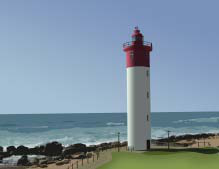
\includegraphics[width=0.245\linewidth]{s1} 
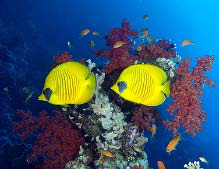
\includegraphics[width=0.245\linewidth]{s2} 
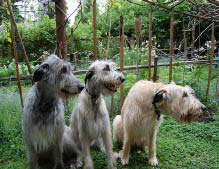
\includegraphics[width=0.245\linewidth]{s3} 
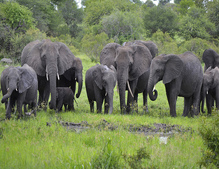
\includegraphics[width=0.245\linewidth]{s4r} 
\end{tikzfigure}
%% \colorlet{innerblockbodybgcolor}{white}
}
\colorlet{innerblockbodybgcolor}{eccvgrayblue}
% More point like?
% the subitizing range modulates the cognitive mechanisms directed at instance counting
\innerblock{}{\boldblue{Subitizing} is a perceptual ability that enables rapid and spontaneous identification of the numerosity of small visual sets. When the \boldblue{subitizing range} of 1 -- 4 instances is exceeded, other cognitive mechanisms related to instance counting are employed. We explore the emergence of visual number sense in unsupervised deep networks trained on \boldblue{natural images} from the \boldblue{Salient Object Subitizing Dataset} \citep{zhang2016salient}. 
% The complexity of natural visual scenes helps capture the abstract nature of number sense.
}
}

\block{VISUAL NUMBER SENSE}{
\colorlet{innerblockbodybgcolor}{white}
\innerblock{}{
%% the one paper (pre-Nieder) with "integral part of the visual world" maybe has figures as well. Reflection of the visiospatial systems... (see paper?) How does the perceptually immediate character of subitizing arise? (visiospatial system)
% "Sudden" character of subitizing
% Cogntive proccesing of indicates , indicating that numerosity is a perceptual category.
% maybe wrapfig works better but couldn't get it to work
\begin{minipage}{0.57\linewidth}
%% \begin{hyphenrules}{nohyphenation}
\begin{itemize}[leftmargin=*, label={\huge\raisebox{-0.25ex}{\textcolor{eccvblue}\textbullet}}]
  \setlength\itemsep{0.5em}
  %% \item Separate systems for exact and approximate numerosity representation
  \item \boldblue{Parallel processing} achieves rapid perceptual discrimination of exact numerosity \citep{dehaene2011number}.
   %% \item Automatic map generation  of salient objects is performed in the visiospatial system.
   \item The visiospatial system performs \boldblue{nonmediated} spatial map generation of salient objects \cite{piazza2009humans}.
  %% \item Subitizing is a \boldblue{nonmediated} process originating in the visiospatial system \cite{piazza2009humans} 
  \item Neural populations can automatically develop the ability to judge visual numerosity.
\end{itemize}
%% \end{hyphenrules}
%% Immediate but limited exact \boldblue{visual numerosity} processing abilities could be a result of a capacity-limited multiple object individuation mechanism that performs \boldblue{parallel processing} of salient objects \citep{poncet2016individuation}. The cause of it's \boldblue{sudden} character is hypothesized to be a byproduct of the visiospatial system's automatic salient object map generation of a limited number of salient locations in the visual field \citep{piazza2009humans}. 
\end{minipage}
\begin{minipage}{0.55\linewidth}
%% \vspace*{-6pt}
\begin{tikzfigure}
  \hspace*{-90pt}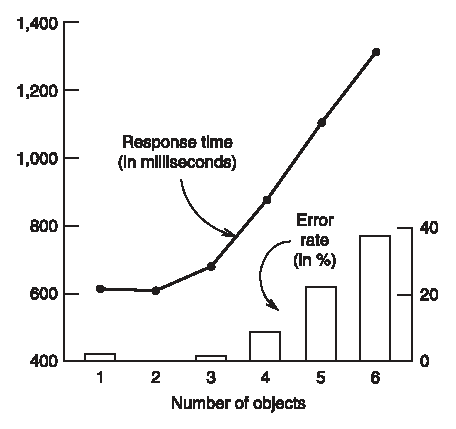
\includegraphics[width=0.75\textwidth]{subcrop}
\end{tikzfigure}
\end{minipage}
}
}

\end{columns}

%% \begin{columns}
%% \column{0.5}
\useblockstyle{eccv2optimizations}
\block{VISUAL OPTIMIZATION RESULTS}{
%% \begin{minipage}[t]{0.4\linewidth}

\useinnerblockstyle{eccvinneroptimizations}
\colorlet{innerblockbodybgcolor}{white}
%% \renewcommand{\columnseprulecolor}{\color[HTML]{E2F1F9}}
%% \setlength{\parskip}{0pt plus 1pt}
%% \setlength{\oddsidemargin}{0pc}
%% \setlength{\marginparwidth}{0pc}
%% \setlength{\topmargin}{0.0pc}
%% \setlength\columnseprule{0.15cm}

%% \setlength\multicolsep{-1.1pt} % this number is dependend on the fontsize

%% \setcounter{columnbadness}{7000}
%% \setcounter{finalcolumnbadness}{7000}
%% \setcounter{collectmore}{-1}
%% \begin{multicols}{2}
\innerblock[bodyinnersep=25pt]{}{
  \centering
  \begin{minipage}{0.494\linewidth}
    \centering
    \begin{tikzfigure}
      \vspace*{-10pt}
      \hspace*{-10pt}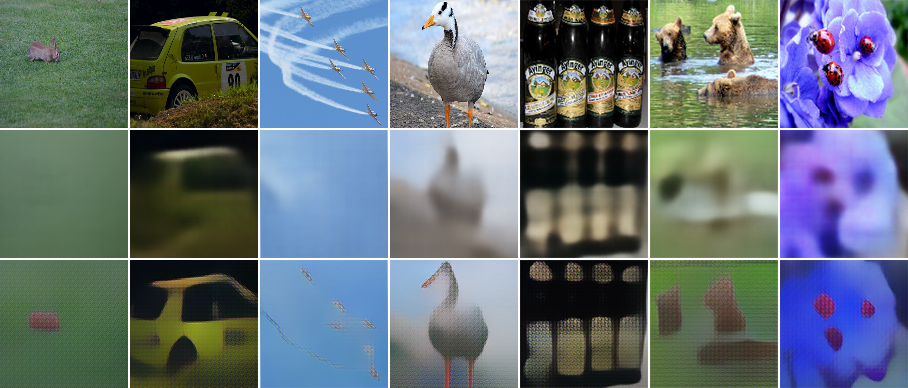
\includegraphics[width=0.8\linewidth]{bce_dfc_crop}
    \end{tikzfigure}
  \end{minipage}\hfill
  \begin{minipage}{0.494\linewidth}
    \centering
    %% \hspace*{45pt}
    \begin{tikzfigure}
      \vspace*{-10pt}
      \hspace*{15pt}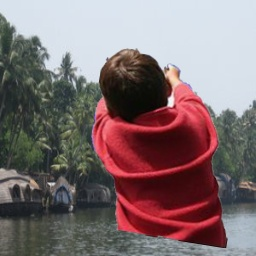
\includegraphics[width=0.175\linewidth]{syn1}\hspace{3pt}%
      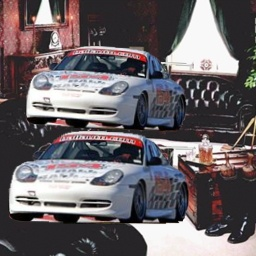
\includegraphics[width=0.175\linewidth]{syn2}\hspace{3pt}%
      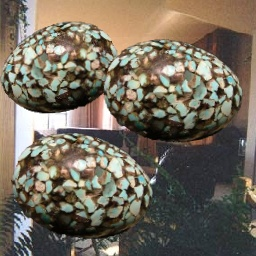
\includegraphics[width=0.175\linewidth]{syn3}\hspace{3pt}%
      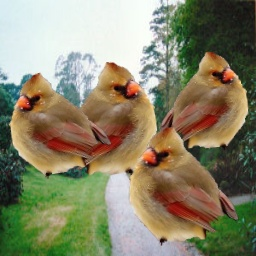
\includegraphics[width=0.175\linewidth]{syn4}\\%
      %% \bigskip
      \vspace*{3pt}
      \hspace*{15pt}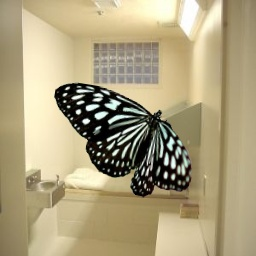
\includegraphics[width=0.175\linewidth]{syn1b}\hspace{3pt}%
      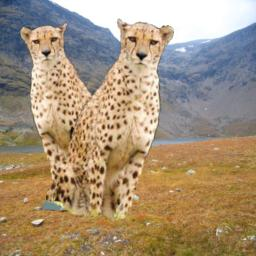
\includegraphics[width=0.175\linewidth]{syn2b}\hspace{3pt}%
      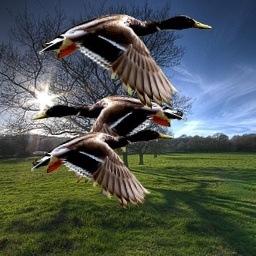
\includegraphics[width=0.175\linewidth]{syn3b}\hspace{3pt}%
      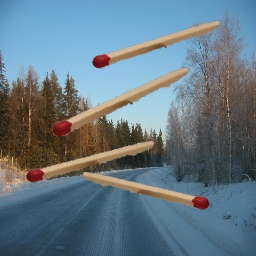
\includegraphics[width=0.175\linewidth]{syn4b}%
    \end{tikzfigure}%
 \end{minipage}%
  
}
\colorlet{innerblockbodybgcolor}{eccvgrayblue}

\useinnerblockstyle{eccvinner}
\innerblock{}{
\renewcommand{\columnseprulecolor}{\color[HTML]{FFFFFF}}
\setlength\columnsep{90pt}
\setlength\columnseprule{0.14cm}
%% \setlength\columnseprule{0.0cm}
\begin{multicols}{2}
% Could drop the first sentence from this block, and the second of the other
{\boldblue{Feature Perceptual Loss} \citep{hou2017deep} improved object contour reconstruction by using intermediate layer representations from a pretrained network in the objective function of the VAE.\par}
{Augmentation of the SOS dataset with \boldblue{synthetic data} was required to familiarize the model with an extensive distribution of object types and the spatial configurations thereof.}
%% \vskip 0.11em
\end{multicols}
}
}

\useblockstyle{eccv2}
\begin{columns}
\column{0.5}


\block{SIZE-INVARIANT NUMEROSITY DETECTORS}{
\colorlet{innerblockbodybgcolor}{white}
\innerblock{}{
  % all tikz figures need slight manual recentering
  % https://tex.stackexchange.com/questions/447615/tikzposter-how-to-center-a-tikzfigure-within-a-block
  \begin{tikzfigure}
    \vspace*{-19pt}
    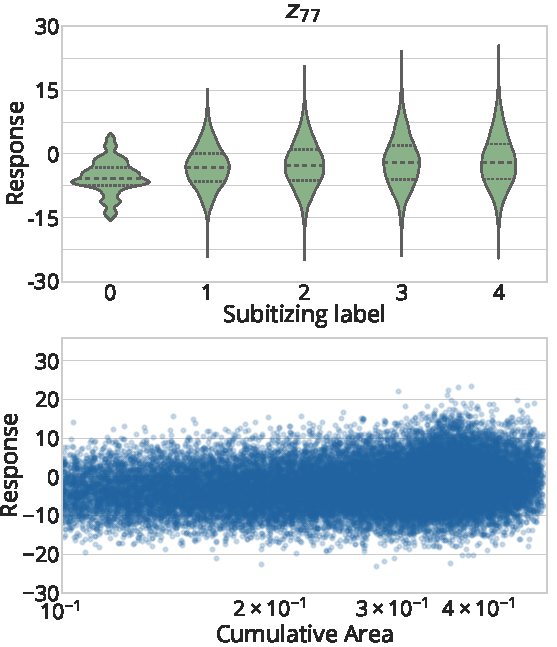
\includegraphics[width=0.40\linewidth]{NN}\hspace{50pt}
    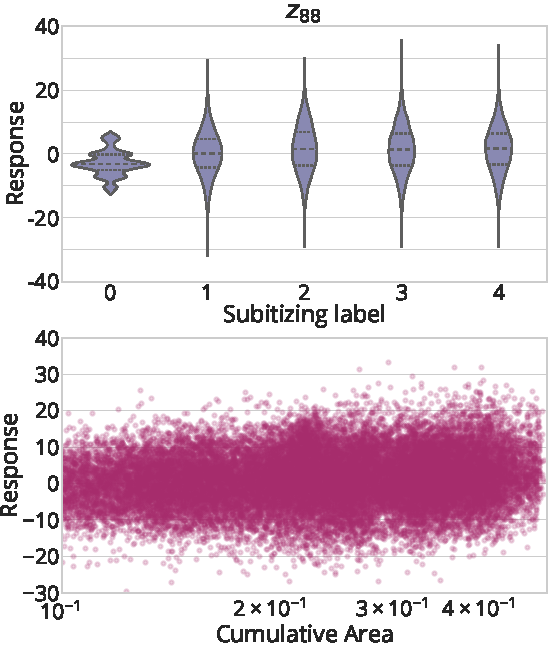
\includegraphics[width=0.40\linewidth]{NA}
  \end{tikzfigure}
}
\colorlet{innerblockbodybgcolor}{eccvgrayblue}
\innerblock{}{
  %% \vspace*{-10pt}
  %% \begin{tikzfigure}
  %%   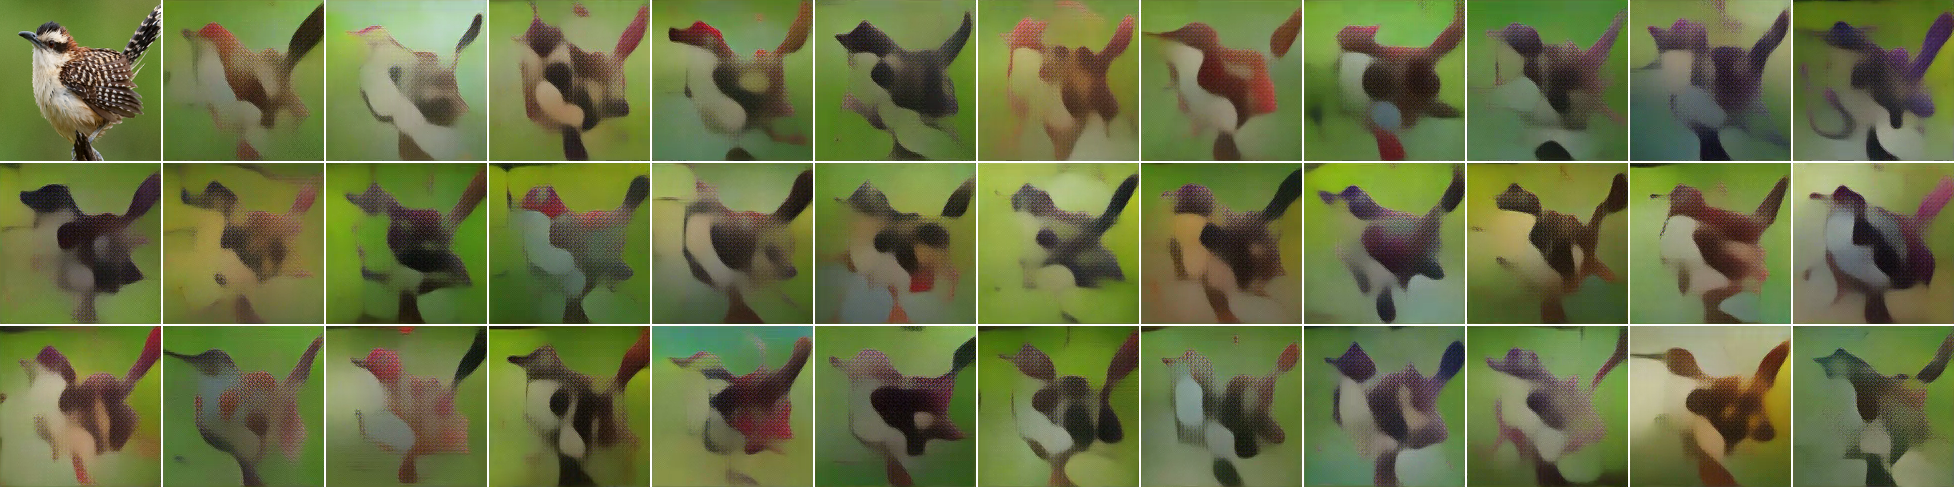
\includegraphics[width=40cm]{bird_varied_crop}
  %% \end{tikzfigure}
  % Reference here?
\vspace*{-20pt}
\begin{tikzfigure}
  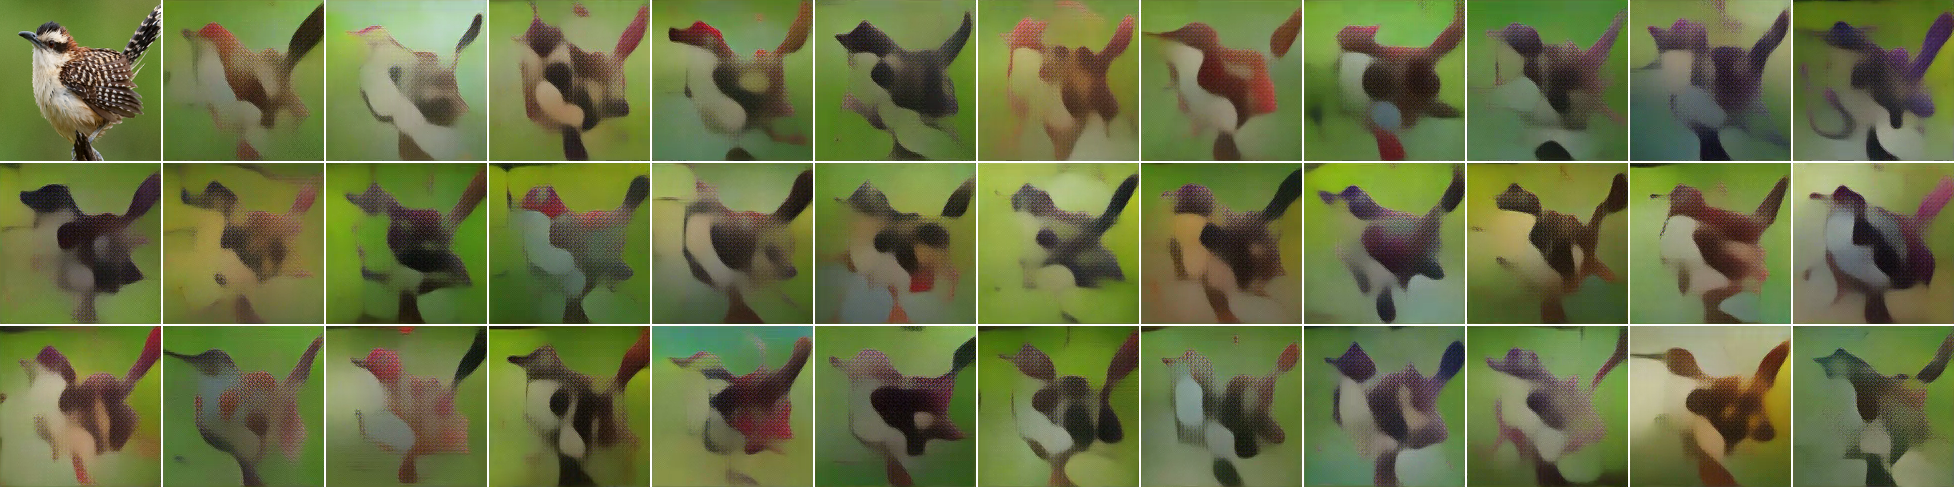
\includegraphics[width=0.39\textwidth]{bird_varied_crop}
\end{tikzfigure}

}
\colorlet{innerblockbodybgcolor}{white}
\innerblock{}{
  Latent dimensions of the learned representations encode complex information, whereby numerosity is likely encoded \boldblue{invariant of cumulative object area}.
 Biological neural networks showcase a similair property.
  %% Comparable with biological neural networks, an analysis of the learned representations revealed that numerosity is represented . However, no latent dimension represents just one visual property. %
}
}

\column{0.5}

\block{SUBITIZING TASK PERFORMANCE}{
\colorlet{innerblockbodybgcolor}{white}
\innerblock{}{
\vspace*{55pt}
\begin{center}
  %% \captionof{table}{Hello world}
  \captionof*{table}{\boldblue{Table:} Average classification precision ({\%}) of count labels across various algorithms.}
\end{center}
\vspace*{-25pt}
\begin{tikzfigure}
    \begin{tabularx}{0.95\linewidth}{lXXXXXX}
    \toprule
    Count Label $\rightarrow$ & \quad 0 & \quad 1 & \quad 2 & \quad 3 & \quad 4+ & \quad mean \\
    \midrule
    %% \rowcolor
    Chance & \quad 27.5 & \quad46.5 & \quad18.6 & \quad11.7 & \quad\phantom{0}9.7 & \quad22.8 \\
    GIST & \quad 67.4 & \quad65.0 & \quad32.3 & \quad17.5 & \quad24.7 & \quad41.4 \\
    SIFT+IFV & \quad 83.0 & \quad68.1 & \quad35.1 & \quad26.6 & \quad38.1 & \quad50.1 \\
    CNN\_FT & \quad 93.6 & \quad93.8 & \quad75.2 & \quad58.6 & \quad71.6 & \quad78.6 \\
    VAE + softmax (ours) & \quad76.0 & \quad49.0 & \quad40.0 & \quad27.0 & \quad30.0 & \quad44.4 \\
    \bottomrule
    \end{tabularx}
\end{tikzfigure}
\vspace*{55pt}
}
\colorlet{innerblockbodybgcolor}{eccvgrayblue}
\innerblock{}{We compare our \boldblue{unsupervised approach} to existing supervised approaches to instance counting. The strength of the representation learned by the VAE is measured by training a simple \boldblue{softmax classifier} that is fed latent representations of images with corresponding count labels.} % numbers are not math font as well
}

\useblockstyle{reference}
% not sure if this actually centers text but it is more centered I guess
 %% screws with the centering
\renewcommand*{\bibfont}{\normalsize}

\block[bodyinnersep=5pt, bodyoffsetx=19pt]{}{
%% \vspace*{15pt}
\noindent\makebox[\linewidth]{\textcolor{lightgrey}{\rule{0.40\paperwidth}{0.12cm}}}
\vspace*{-39pt}
{
  %% \begin{center}
    %% \begin{minipage}{0.94\linewidth}
    % maybe print as /small text
    {
      \bibliography{poster}
      %% \printbibliography[heading=none]
    }
    %% \end{minipage}
  %% \end{center}
}
}

\end{columns}

%


\end{document}
